\documentclass{beamer}
\usetheme{Boadilla}
\usecolortheme{sidebartab}

\usepackage{hyperref}
\usepackage{showexpl} 
\usepackage{graphicx}
\usepackage{color}
\usepackage{siunitx}
\usepackage[version=3]{mhchem}
\usepackage{chemfig}
\usepackage{changes}
\usepackage[many]{tcolorbox}
\usepackage{natbib}
\bibliographystyle{unsrtnat}
\setcitestyle{square,numbers}

\beamertemplatenavigationsymbolsempty
\setbeamertemplate{footline}{}
\setbeamertemplate{bibliography item}{\insertbiblabel}

\lstloadlanguages{[LaTeX]Tex} 
\lstset{% 
     basicstyle=\ttfamily\large, 
     commentstyle=\itshape\ttfamily, 
     showspaces=false, 
     showstringspaces=false, 
     breaklines=true, 
     breakautoindent=false, 
     captionpos=t,
     explpreset={numbers=none},
     pos=b
} 

\title{Working with Research Data}
\author{Markus Stocker}
\date{September 12, 2017}

\begin{document}

\maketitle

\begin{frame}
  \frametitle{Outline}
  
  \begin{itemize}
  \item Accessing and reusing research data
  \item Computational environments for data processing
  \item Curating and storing data, from files to databases
  \item Research data versioning and backup
  \end{itemize}
\end{frame}

\begin{frame}
  \frametitle{Data Access}
  
  \begin{itemize}
  \item It's complicated but it is improving
  \item Drivers for better access
  \begin{itemize}
  \item Open Data imperative
  \item Credit for publishing data
  \item Increase return on investment in scientific research
  \item Funders requiring data to be published
  \end{itemize}
  \item Correspondingly, supporting infrastructures is
  \begin{itemize}
  \item Increasing in number and quality
  \item Adopting principles, guidelines, standards
%  \item Supporting human and programmatic access
  \end{itemize}
  \end{itemize}
\end{frame}

\begin{frame}
  \frametitle{Data Access}
  
  \begin{itemize}
  \item You know how to access \emph{your} data
  \item More difficult is access to data authored by others
  \item Presumes others have published their data
  \item Then you may be able to
  \begin{itemize}
  \item Find their data
  \item Retrieve the data
  \item Reuse the data
  \end{itemize}
  \end{itemize}
\end{frame}

\begin{frame}
  \frametitle{Find Data}
  
  \begin{itemize}
  \item Useful data can be found in a lot of places
  \item Online or offline, e.g. printed books
  \item In data repositories or as files on a server
  \item You could try a Google search
  \item Or ask your supervisor and fellow students
  \item The authors of papers you read may cite data and/or sources
%  \item Specialized search, e.g. Registry of Research Data Repositories
  \end{itemize}
\end{frame}

{
	\usebackgroundtemplate{ %
		\begin{tikzpicture}[remember picture, overlay]%
		\node at (current page.center) {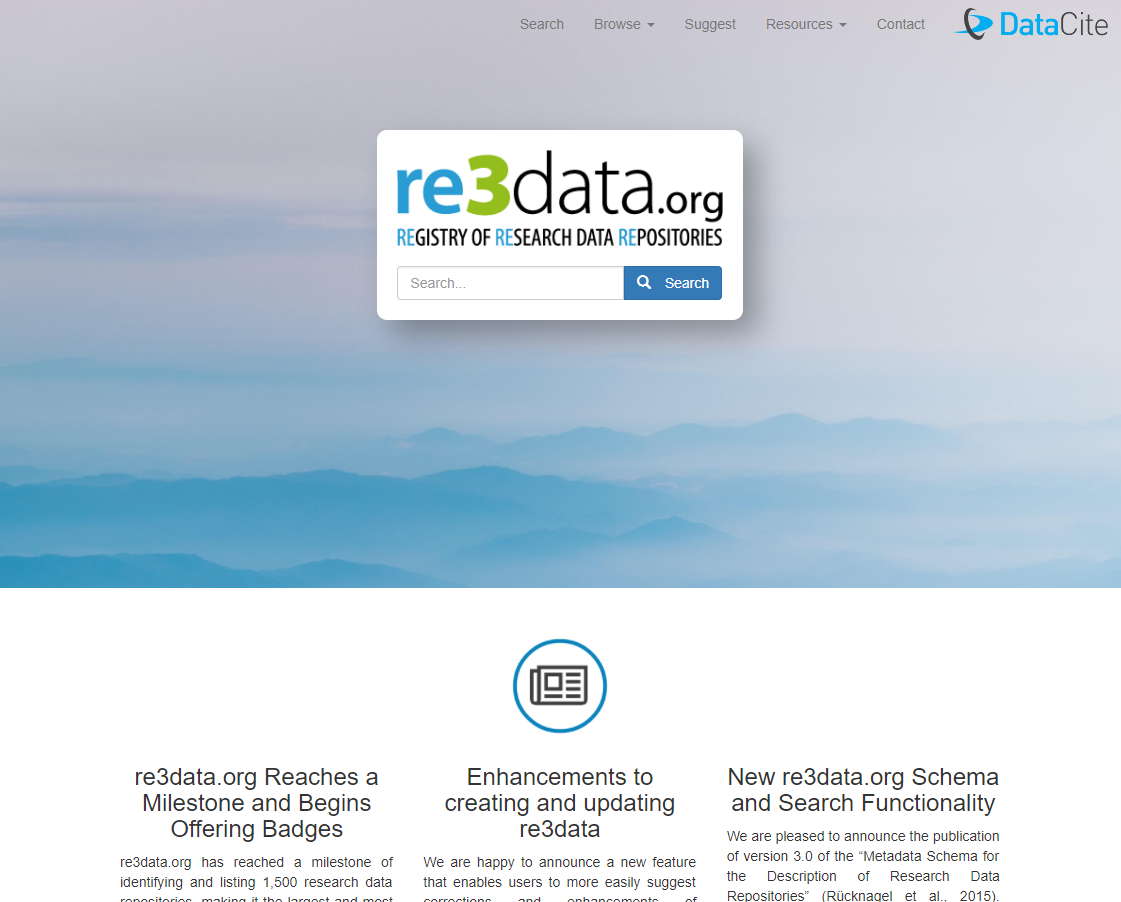
\includegraphics[height=\paperheight]{graphics/re3dataorg.png}};%
		\end{tikzpicture}%
	}%
	\setbeamertemplate{navigation symbols}{}
	\begin{frame}[plain]
	\end{frame}
}

{
	\usebackgroundtemplate{ %
		\begin{tikzpicture}[remember picture, overlay]%
		\node at (current page.center) {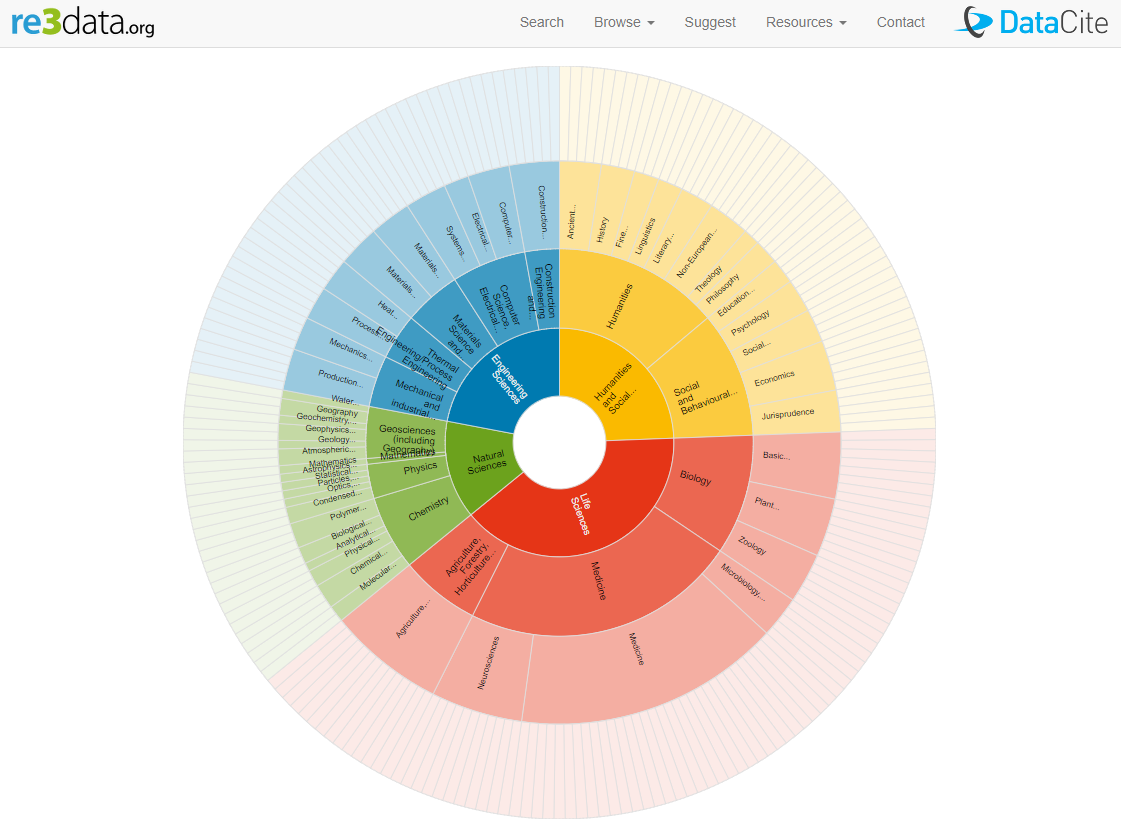
\includegraphics[height=\paperheight]{graphics/re3dataorg-subjects.png}};%
		\end{tikzpicture}%
	}%
	\setbeamertemplate{navigation symbols}{}
	\begin{frame}[plain]
	\end{frame}
}

\begin{frame}
  \frametitle{Retrieve Data}
  
  \begin{itemize}
  \item Typically download of one or more files
  \item An API for programmatic retrieval may be available
  \item Data repositories generally support search
  \item Often data are retrieved as they were deposited (original format)
  \item Repository may standardize data during ingestion
  \end{itemize}
\end{frame}

{
	\usebackgroundtemplate{ %
		\begin{tikzpicture}[remember picture, overlay]%
		\node at (current page.center) {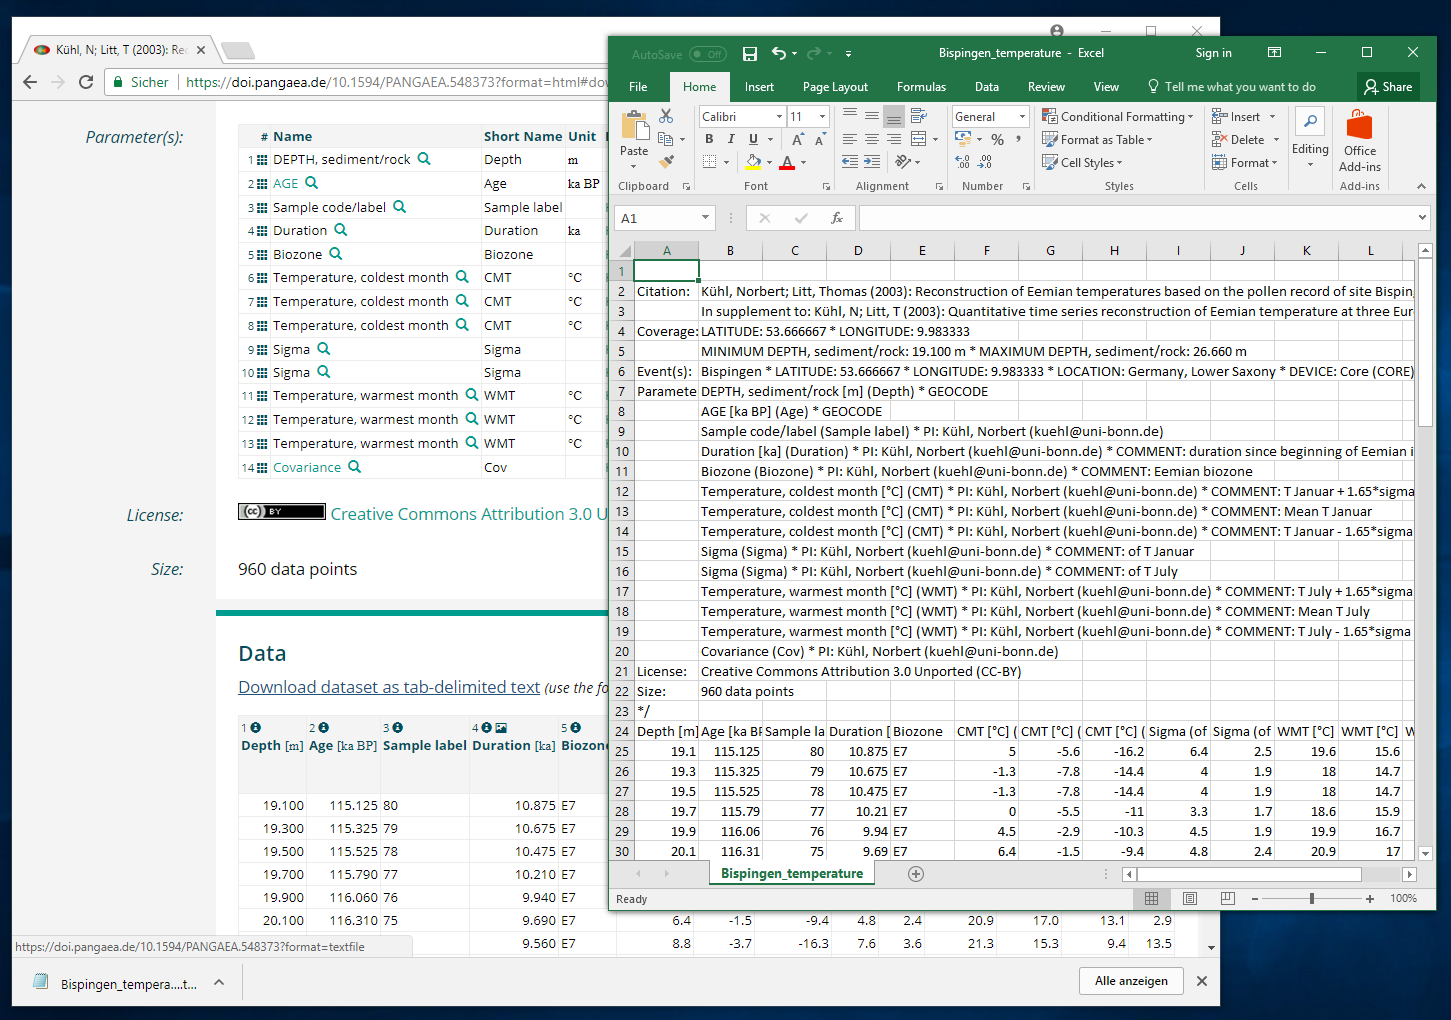
\includegraphics[width=\paperwidth]{graphics/pangaea-download.png}};%
		\end{tikzpicture}%
	}%
	\setbeamertemplate{navigation symbols}{}
	\begin{frame}[plain]
	\end{frame}
}

\begin{frame}
  \frametitle{Reuse Data}
  
  \begin{itemize}
  \item Complicated!
  \item Generally substantial processing needed to make reuse possible
  \item Even if accessible, data are generally not interoperable
  \item Lack syntactic interoperability due to different formats
  \item Lack semantic interoperability due to different terminology
  \item Data and metadata quality may not be adequate
  \item Different resolution, gaps, outliers, insufficient information, ...
%  \item Data need to be integrated: common syntax and semantics
%  \item A lot of time required to prepare for reuse
  \end{itemize}
\end{frame}

\begin{frame}
  \frametitle{Data Processing}
  
  \begin{itemize}
  \item Assume integrated data
  \item Your next step is to process them for your purpose
  \item Staggering amount of methods
  \item Programming (scripting) languages
  \item Computational environments and other tools
  \item Processing results in new (derived) data
  \item Various kinds of processing, transformation, interpretation, ...
  \end{itemize}
\end{frame}

\begin{frame}
  \frametitle{Curating and Storing Data}
  
  \begin{itemize}
  \item Data need to be identified, described, quality controlled, etc.
  \item Curated data are stored and possibly preserved
  \item How you curate and store data depends on various factors, e.g.
  \begin{itemize}
  \item Longevity: temporary vs. preserved data
  \item Sharing: yourself vs. community
  \item Dynamism: static files vs. streamed data
  \end{itemize}
  \end{itemize}
\end{frame}

{
	\usebackgroundtemplate{ %
		\begin{tikzpicture}[remember picture, overlay]%
		\node[at=(current page.south east), anchor=south east,inner sep=20pt]  {
\includegraphics[scale=0.2]{graphics/postgresql.png}};%
		\end{tikzpicture}%
	}%
	\setbeamertemplate{navigation symbols}{}
	\begin{frame}[plain]
	  \frametitle{Databases}
	  
	  \begin{itemize}
	  \item Many kinds but relational most common
	  \item Help structuring data, be consistent with datatypes
	  \item Flexible data retrieval with declarative language (SQL)
	  \item Access to data from programming languages (Python, R, Java, ...)
	  \item Processing of large data quantities
	  \item Access management and security
	  \item Backup
	  \end{itemize}
	\end{frame}
}

\begin{frame}[fragile]
  \frametitle{Databases}
  
  \small
  \begin{verbatim}
create table data (
  id integer primary key, 
  time timestamp, 
  latitude double precision, 
  longitude double precision, 
  temperature double precision
)
  \end{verbatim}
\end{frame}

\begin{frame}[fragile]
  \frametitle{Databases}
  
  \small
  \begin{verbatim}
insert into data values(
  1, 
  timestamp '2016-07-26 00:00:00', 
  -70.650000, 
  -8.250000, 
  -19.3
)
  \end{verbatim}
\end{frame}

\begin{frame}[fragile]
  \frametitle{Databases}
  
  \small
  \begin{verbatim}
select 
  id, time, latitude, longitude, temperature
from data
  
select * from data where temperature < -15
  
  
  
  id |        time         | latitude | longitude | temperature 
 ----+---------------------+----------+-----------+-------------
   1 | 2016-07-26 00:00:00 |   -70.65 |     -8.25 |       -19.3 
  \end{verbatim}
\end{frame}

\begin{frame}[fragile]
  \frametitle{From Python}
  
  \small
  \begin{verbatim}
import pyodbc

con = pyodbc.connect('DRIVER=...;SERVER=...;PORT=...;
                      DATABASE=...;UID=...;PWD=...')
cur = con.cursor()

cur.execute('select latitude, longitude, temperature 
             from data where temperature < -15')

for row in cur.fetchall():
  print('Latitute: {}; Longitude: {}; Temperature: {}'
        .format(row[0], row[1], row[2])

cur.close()
con.close()
  \end{verbatim}
\end{frame}

\begin{frame}
  \frametitle{Backup and Versioning}
  
  \begin{itemize}
  \item Your (Word) manuscripts are data
  \item Backup your other data as you backup your manuscripts
%  \item Avoid memory sticks as backup media
  \item Test your backup strategy: can you recover lost files?
  \item Consider to version your data
  \item Including if you collaborate only with yourself
  \item Remote version control can act as backup
  \end{itemize}
\end{frame}

\begin{frame}
  \frametitle{Take aways}
  
  \begin{itemize}
    \item Reusing data depends on publishing, finding and access
    \item They all have their challenges
    \item Preparing data for reuse is generally laborious
    \item Don't forget curation, storage beyond research project
    \item Remember backup, versioning, even to collaborate with yourself
  \end{itemize}
\end{frame}

\end{document}
